%%%%%%%%%%%%%%%%%%%%%%%%%%%%%%%%%%%%%%%%%%%%%%%%%%%%%%%%%%%%%%%%%%%%%%%%%%%%%%%%%%
\begin{frame}[fragile]\frametitle{}
\begin{center}
{\Large Applications}
\end{center}
\end{frame}

%%%%%%%%%%%%%%%%%%%%%%%%%%%%%%%%%%%%%%%%%%%%%%%%%%%%%%%%%%%%%%%%%%%%%%%%%%%%%%%%%%
\begin{frame}[fragile]\frametitle{Explain Complex Subjects}
\begin{center}
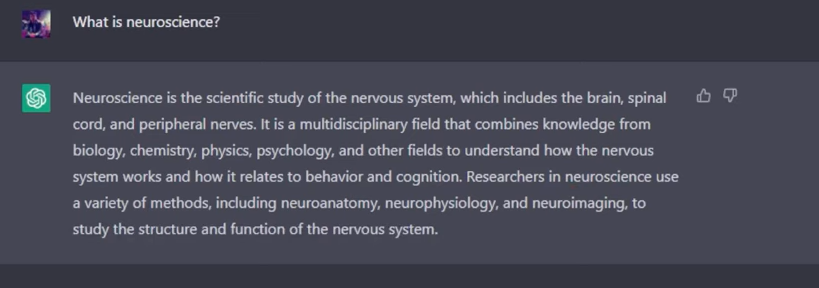
\includegraphics[width=\linewidth,keepaspectratio]{chatgpt15}
\end{center}
	
{\tiny (Ref: Top 10 Chat GPT Use Cases - Simplilearn)}
\end{frame}

%%%%%%%%%%%%%%%%%%%%%%%%%%%%%%%%%%%%%%%%%%%%%%%%%%%%%%%%%%%%%%%%%%%%%%%%%%%%%%%%%%
\begin{frame}[fragile]\frametitle{Write Code}
\begin{center}
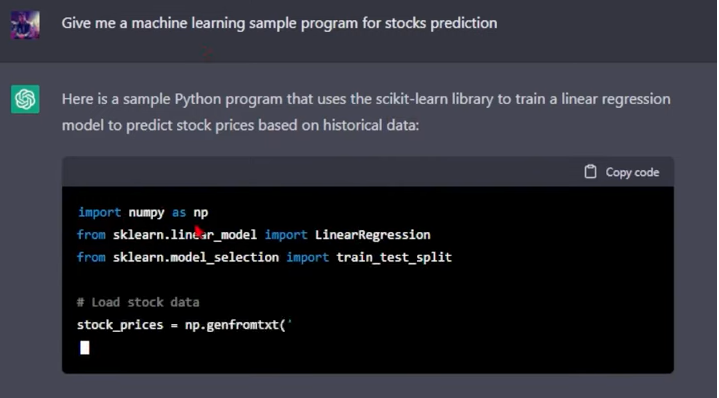
\includegraphics[width=0.8\linewidth,keepaspectratio]{chatgpt16}
\end{center}

it was still writing but I stopped it, just to show this pic

{\tiny (Ref: Top 10 Chat GPT Use Cases - Simplilearn)}
\end{frame}

%%%%%%%%%%%%%%%%%%%%%%%%%%%%%%%%%%%%%%%%%%%%%%%%%%%%%%%%%%%%%%%%%%%%%%%%%%%%%%%%%%
\begin{frame}[fragile]\frametitle{Debug Code}
\begin{center}
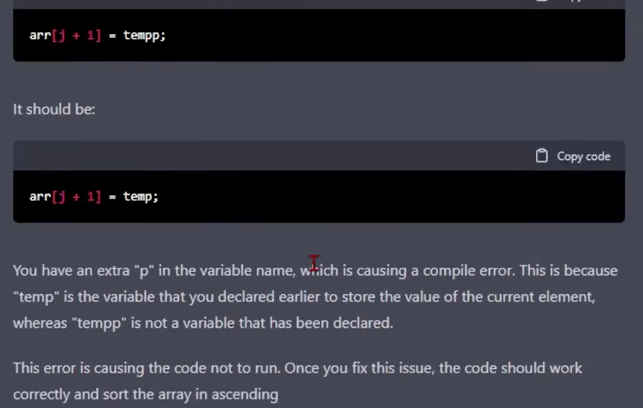
\includegraphics[width=0.8\linewidth,keepaspectratio]{chatgpt17}
\end{center}

{\tiny (Ref: Top 10 Chat GPT Use Cases - Simplilearn)}
\end{frame}

%%%%%%%%%%%%%%%%%%%%%%%%%%%%%%%%%%%%%%%%%%%%%%%%%%%%%%%%%%%%%%%%%%%%%%%%%%%%%%%%%%
\begin{frame}[fragile]\frametitle{Get Custom Marketing Strategy}
\begin{center}

\includegraphics[width=\linewidth,keepaspectratio]{chatgpt18}
\end{center}

{\tiny (Ref: Top 10 Chat GPT Use Cases - Simplilearn)}
\end{frame}

%%%%%%%%%%%%%%%%%%%%%%%%%%%%%%%%%%%%%%%%%%%%%%%%%%%%%%%%%%%%%%%%%%%%%%%%%%%%%%%%%%
\begin{frame}[fragile]\frametitle{Write Articles}
\begin{center}
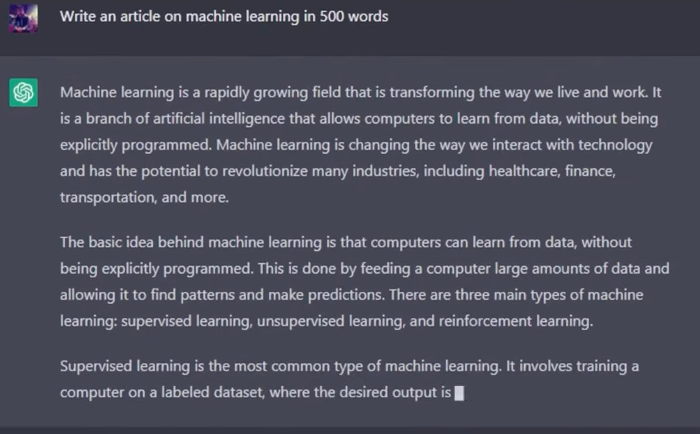
\includegraphics[width=\linewidth,keepaspectratio]{chatgpt19}
\end{center}

{\tiny (Ref: Top 10 Chat GPT Use Cases - Simplilearn)}
\end{frame}

%%%%%%%%%%%%%%%%%%%%%%%%%%%%%%%%%%%%%%%%%%%%%%%%%%%%%%%%%%%%%%%%%%%%%%%%%%%%%%%%%%
\begin{frame}[fragile]\frametitle{Summarize Book}
\begin{center}
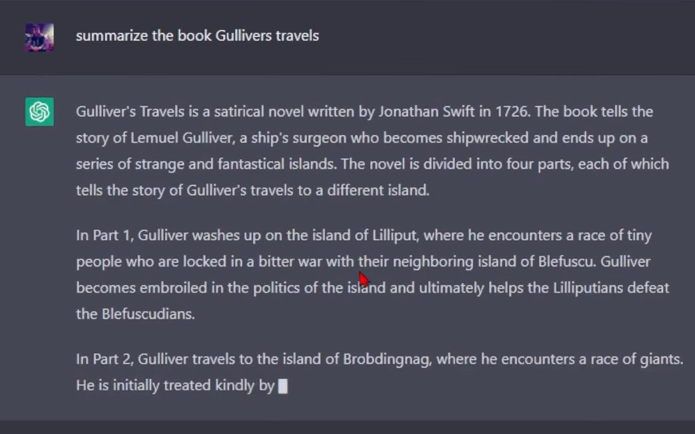
\includegraphics[width=\linewidth,keepaspectratio]{chatgpt20}
\end{center}

{\tiny (Ref: Top 10 Chat GPT Use Cases - Simplilearn)}
\end{frame}

%%%%%%%%%%%%%%%%%%%%%%%%%%%%%%%%%%%%%%%%%%%%%%%%%%%%%%%%%%%%%%%%%%%%%%%%%%%%%%%%%%
\begin{frame}[fragile]\frametitle{Answer Interview Questions}
\begin{center}
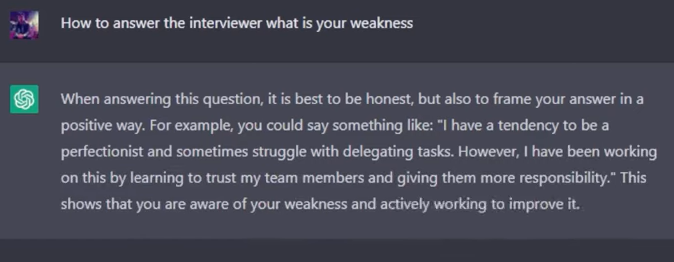
\includegraphics[width=\linewidth,keepaspectratio]{chatgpt21}
\end{center}

{\tiny (Ref: Top 10 Chat GPT Use Cases - Simplilearn)}
\end{frame}



%%%%%%%%%%%%%%%%%%%%%%%%%%%%%%%%%%%%%%%%%%%%%%%%%%%%%%%%%%%%%%%%%%%%%%%%%%%%%%%%%%
\begin{frame}[fragile]\frametitle{Develop Apps}
\begin{center}
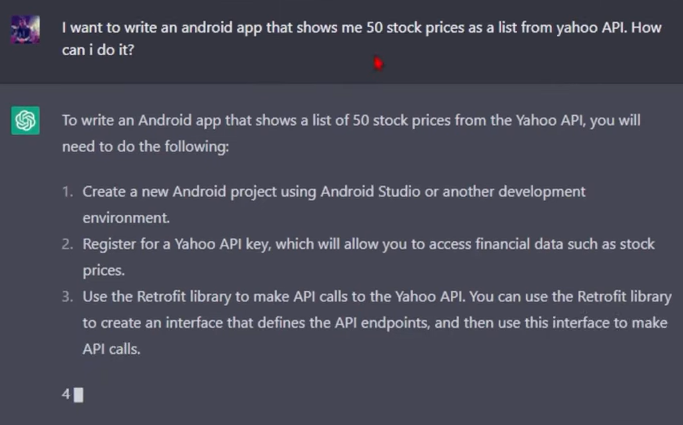
\includegraphics[width=\linewidth,keepaspectratio]{chatgpt22}
\end{center}

{\tiny (Ref: Top 10 Chat GPT Use Cases - Simplilearn)}
\end{frame}

%%%%%%%%%%%%%%%%%%%%%%%%%%%%%%%%%%%%%%%%%%%%%%%%%%%%%%%%%%%%%%%%%%%%%%%%%%%%%%%%%%
\begin{frame}[fragile]\frametitle{Create Health Plan}
\begin{center}
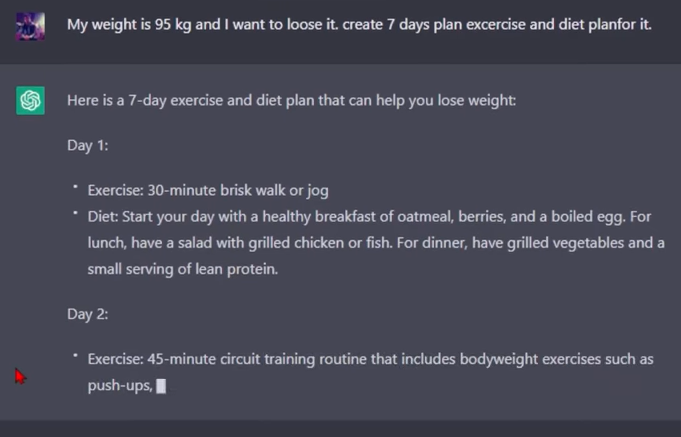
\includegraphics[width=\linewidth,keepaspectratio]{chatgpt23}
\end{center}

{\tiny (Ref: Top 10 Chat GPT Use Cases - Simplilearn)}
\end{frame}

%%%%%%%%%%%%%%%%%%%%%%%%%%%%%%%%%%%%%%%%%%%%%%%%%%%%%%%%%%%%%%%%%%%%%%%%%%%%%%%%%%
\begin{frame}[fragile]\frametitle{Answer General Knowledge Questions}
\begin{center}
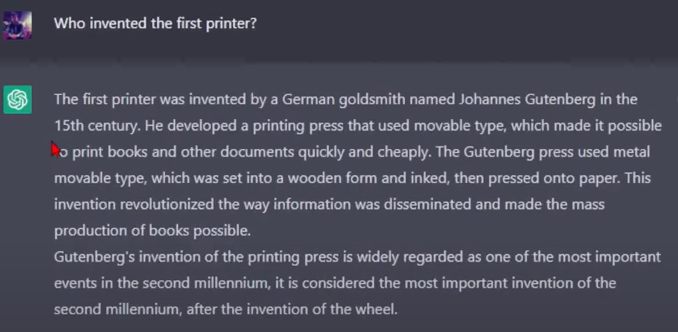
\includegraphics[width=\linewidth,keepaspectratio]{chatgpt24}
\end{center}

{\tiny (Ref: Top 10 Chat GPT Use Cases - Simplilearn)}
\end{frame}


%%%%%%%%%%%%%%%%%%%%%%%%%%%%%%%%%%%%%%%%%%%%%%%%%%%%%%%%%%%%%%%%%%%%%%%%%%%%%%%%%%
\begin{frame}[fragile]\frametitle{Advanced Prompts}
\begin{itemize}
    \item  Five Whys Technique: ``Act like a Root Cause Analyst. Begin by identifying the problem related to [topic]. Now, ask 'why?' this problem exists. Repeat the question 'why?' four more times, digging deeper into each layer to uncover the root cause. Summarize your findings and suggest potential solutions.''
	\item TRIZ (Theory of Inventive Problem Solving): "Act like an Inventive Problem Solver. Utilize TRIZ principles to systematically solve problems related to [topic]. Identify contradictions and apply inventive principles to resolve them. Outline your steps and findings, explaining how the TRIZ methodology was applied."
	\item Job-To-Be-Done Framework: "Act like a Customer Insight Specialist. Examine [topic] through the Job-To-Be-Done lens, exploring the underlying 'jobs' customers are 'hiring' the product or service to accomplish. Detail the customer needs, contexts, and pain points. Propose alignment strategies to meet these 'jobs.'"
	\item Ishikawa Diagram (Fishbone Diagram): "Act like a Quality Improvement Specialist. Build an Ishikawa diagram to explore the causes of a problem related to [topic]. Break down each main branch into finer details, exploring root causes and relationships. Provide insights into potential solutions and preventive measures."
\end{itemize}

{\tiny (Ref: LinkedIn Post - Ruben Hassid)}
\end{frame}

%%%%%%%%%%%%%%%%%%%%%%%%%%%%%%%%%%%%%%%%%%%%%%%%%%%%%%%%%%%%%%%%%%%%%%%%%%%%%%%%%%
\begin{frame}[fragile]\frametitle{Advanced Prompts}
\begin{itemize}
    \item Zwicky Box (Morphological Analysis): "Act like a Complex Systems Analyst. Utilize a Zwicky Box to systematically explore all possible solutions for [topic]. Define dimensions, attributes, and interactions within the system. Explain how you developed the combinations and their relevance to [topic]."
    \item Affinity Diagram: "Act like an Organizational Psychologist. Organize ideas related to [topic] into an affinity diagram. Group concepts by natural relationships, providing explanations for each category. Analyze the groupings and how they provide a coherent understanding of [topic]."
    \item Ansoff Matrix: "Act like a Growth Strategist. Utilize the Ansoff Matrix to explore growth strategies for [topic]. Assess opportunities for market penetration, market development, product development, and diversification. Explain the rationale for each strategy and propose an implementation plan."
    \item Impact/Effort Matrix: "Act like a Project Management Expert. Plot ideas related to [topic] on an impact/effort matrix. Analyze the strategies that should be prioritized, considering both their potential impact and required effort. Provide a systematic plan for execution, including risk assessment."
\end{itemize}

{\tiny (Ref: LinkedIn Post - Ruben Hassid)}
\end{frame}

% %%%%%%%%%%%%%%%%%%%%%%%%%%%%%%%%%%%%%%%%%%%%%%%%%%%%%%%%%%%%%%%%%%%%%%%%%%%%%%%%%%
% \begin{frame}[fragile]\frametitle{HVAC QnA}
% Prompt: ``Diagnose a frosted evaporator coil''

% Result: 
% ``There are several reasons why an evaporator coil may become frosted:
% \begin{itemize}
% \item Low refrigerant levels: If the refrigerant levels in the system are too low, it can cause the
% evaporator coil to freeze. This is because the refrigerant is responsible for absorbing heat
% from the air, and without enough refrigerant, the coil will not be able to absorb enough heat
% to prevent freezing.
% \item Dirty air filter: A dirty air filter can restrict airflow to the evaporator coil, causing the coil
% to freeze.
% \item Blocked or restricted airflow: If the airflow to the evaporator coil is blocked or
% restricted, the coil may freeze. This can be caused by a number of things such as dirty ducts or
% registers, closed or blocked vents, or a malfunctioning blower fan.
% \item Obstruction in the drain line: A blockage in the drain line can cause water to back up and freeze on the coil.
% \end{itemize}	 
% It's important to fix the issue as soon as possible, as a frozen evaporator coil can lead to decreased
% efficiency and can cause damage to the unit.
% ''

% \tiny{(Ref:ChatGPT Could Be the 'Write' Choice for HVACR Contractors - Joanna R. Turpin)}
% \end{frame}

% %%%%%%%%%%%%%%%%%%%%%%%%%%%%%%%%%%%%%%%%%%%%%%%%%%%%%%%%%%%%%%%%%%%%%%%%%%%%%%%%%%
% \begin{frame}[fragile]\frametitle{HVAC QnA}
% Prompt: ``How to respond to a customer who thinks an air conditioner is
% too expensive''

% Result: ``
% \begin{itemize}
% \item Understand their concerns: Find out why they think the air conditioner is too expensive.
% Are they comparing it to a lower-quality unit? Are they on a tight budget? Understanding
% their concerns will help you address them more effectively.
% \item Provide a detailed explanation of the costs: Explain the costs associated with the air
% conditioner, including the cost of the unit, installation, and any additional materials or labor
% that may be required.
% \item Compare costs with the benefits: Explain the benefits of the air conditioner, such as
% energy efficiency, durability, and long-term cost savings. Explain how the cost of the unit may
% be offset by energy savings in the long run.
% \item Offer financing options: If the customer is unable to afford the air conditioner upfront,
% offer financing options that can help them spread the cost over time.

% \end{itemize}	 

% \ldots

% \tiny{(Ref:ChatGPT Could Be the 'Write' Choice for HVACR Contractors - Joanna R. Turpin)}
% \end{frame}

% %%%%%%%%%%%%%%%%%%%%%%%%%%%%%%%%%%%%%%%%%%%%%%%%%%%%%%%%%%%%%%%%%%%%%%%%%%%%%%%%%%
% \begin{frame}[fragile]\frametitle{HVAC QnA}

% \ldots 

% \begin{itemize}
% \item Provide a written estimate: Provide the customer with a detailed, written estimate that
% outlines the costs associated with the air conditioner and the benefits it will provide. This will
% help them make an informed decision.
% \item Provide a guarantee or warranty on the unit: Provide the customer with a guarantee
% or warranty on the unit to give them peace of mind in their investment.
% \item Provide an alternative solution: If the customer cannot afford the recommended
% solution, offer an alternative solution that fits their budget while still meeting their needs.
% \end{itemize}	 
% It's important to be patient, understanding and provide all the information customers need to
% make a decision that best fits their needs and budget.
% ''

% \tiny{(Ref:ChatGPT Could Be the 'Write' Choice for HVACR Contractors - Joanna R. Turpin)}
% \end{frame}

% %%%%%%%%%%%%%%%%%%%%%%%%%%%%%%%%%%%%%%%%%%%%%%%%%%%%%%%%%%%%%%%%%%%%%%%%%%%%%%%%%%
% \begin{frame}[fragile]\frametitle{If This Then That}


% \begin{itemize}
% \item With well designed prompts, one can format output in json (read, key-value pairs)
% \item Parsing via python program, one can trigger Actions. (GPT3 APIs for now)
% \item Whole pipeline can be put in place programmatically, doing any trigger based work (IFTTT - If This Then That)
% \end{itemize}	 


% \tiny{(Ref: ChatGPT for Arduino - MoonPreneur)}
% \end{frame}

% %%%%%%%%%%%%%%%%%%%%%%%%%%%%%%%%%%%%%%%%%%%%%%%%%%%%%%%%%%%%%%%%%%%%%%%%%%%%%%%%%%
% \begin{frame}[fragile]\frametitle{Possible applications}



% \begin{itemize}
% \item Multi-Language Support: ChatGPT�s ability to translate languages can be combined with Arduino to create multi-language support for devices. This feature makes it possible for users from different countries to interact with the device in their language. For example, you can create a device that provides information about local tourist attractions and supports multiple languages.
% \item Home Automation: One unique application of this combination is in the field of home automation. With ChatGPT�s ability to understand and respond to natural language and the versatility of the Arduino platform, it�s possible to create a fully voice-controlled smart home system. 
% \end{itemize}	 



% \tiny{(Ref: ChatGPT for Arduino - MoonPreneur)}
% \end{frame}

%%%%%%%%%%%%%%%%%%%%%%%%%%%%%%%%%%%%%%%%%%%%%%%%%%%%%%%%%%%%%%%%%%%%%%%%%%%%%%%%%%
\begin{frame}[fragile]\frametitle{AI Transforming Finance}
There are five key areas where AI can bring transformative changes to finance:
\begin{itemize}
    \item Personalize services and products
    \item Create new opportunities
    \item Manage risk and fraud
    \item Enable transparency and compliance
    \item Automate operations and reduce costs
\end{itemize}
\end{frame}

%%%%%%%%%%%%%%%%%%%%%%%%%%%%%%%%%%%%%%%%%%%%%%%%%%%%%%%%%%%%%%%%%%%%%%%%%%%%%%%%%%
\begin{frame}[fragile]\frametitle{AI in Finance: Examples}
\textbf{Personalizing Services \& Products}
\begin{itemize}
    \item Morgan Stanley: Next Best Action AI engine for tailored client messages.
    \item Klarna: Uses ChatGPT for personalized shopping suggestions.
\end{itemize}

\textbf{Creating New Opportunities}
\begin{itemize}
    \item Citadel: Negotiating enterprise-wide license for OpenAI's ChatGPT.
    \item Deutsche Bank: AI applications with NVIDIA for risk management and efficiency.
\end{itemize}

\textbf{Enabling Transparency \& Compliance}
\begin{itemize}
    \item Flagright: Introduces Flagright AI suite for global AML compliance.
\end{itemize}

\textbf{Automating Operations \& Reducing Costs}
\begin{itemize}
    \item JPMorgan: Developing IndexGPT for AI-driven financial recommendations.
\end{itemize}
\end{frame}


%%%%%%%%%%%%%%%%%%%%%%%%%%%%%%%%%%%%%%%%%%%%%%%%%%%%%%%%%%%%%%%%%%%%%%%%%%%%%%%%%%
\begin{frame}[fragile]\frametitle{Applications to Finance}
\begin{center}
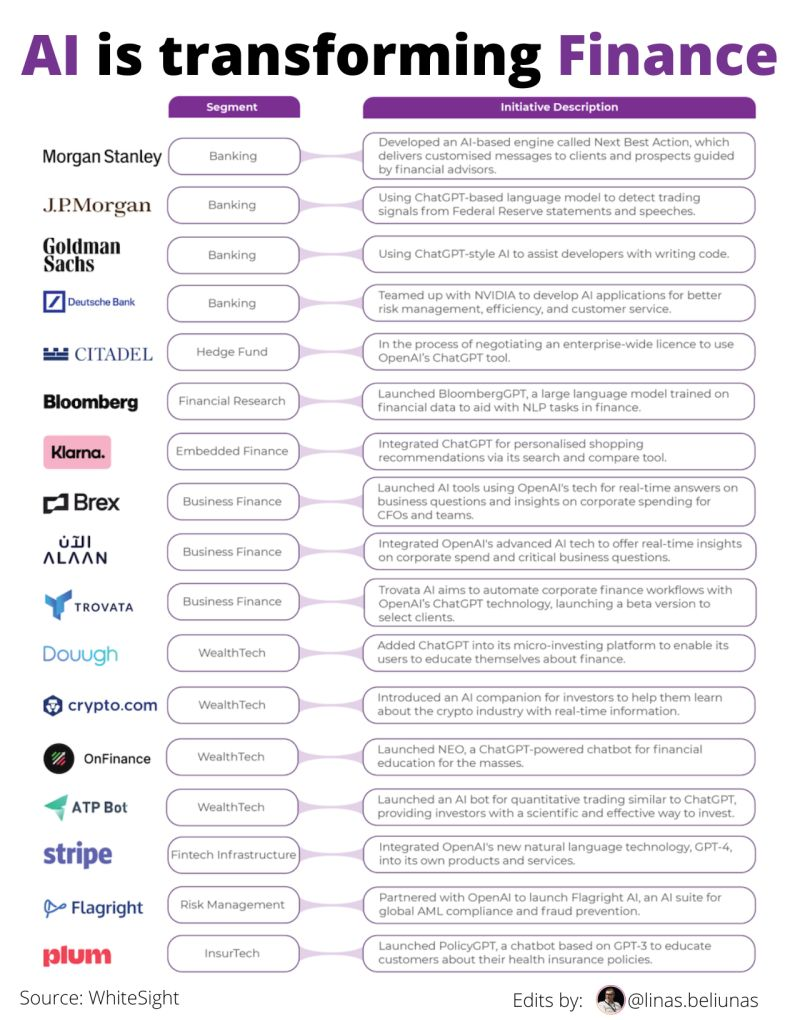
\includegraphics[width=0.8\linewidth,keepaspectratio]{llm91}
\end{center}

{\tiny (Ref: LinkedIn Post - Linas Beliunas)}
\end{frame}
